\documentclass{tk3-team}
\usepackage[caption=false,font=footnotesize]{subfig}


\begin{document}

\Ex{iLift}{\today}{Group G}%
                {Elmi Ali}{Satia Herfert}%
                {Omar Erminy}{Floriment Klinaku}%
                {Yiqun Chen}%

\section{Problem statement}

When going to the gym, one often faces problems that are hard to solve without ubiquitous technology. In order to make progress, it is essential to keep track of
\begin{itemize}
	\item what equipment you used,
	\item how much weight you used,
	\item what exercises you did,
	\item how many repetitions you did, and
	\item how well you performed the exercise.
\end{itemize}

The conventional solution would be to use pen and paper to write down your sessions, or use your smartphone for the same purpose. Usually people are too lazy to write down information about each set in detail and just write down how many sets they did with what weight, at most.

More problems with this are that you have keep track manually which hinders the training flow, and that you have to look for the right information in a probably suboptimal representation (not a table) on your paper. Some graphs displaying different statistics would also be very helpful so you can see your progress in a fast and descriptive way.

In addition, when using a paper, you don't have access to your statistics anywhere outside of the gym. If you want to train somewhere else, like at home, in a different city, or outside, that can be a big obstacle.

In order to know how well you performed each exercise you need a lot of experience or advice from a professional. Sadly, few gyms provide personal trainers that assist your, or that service is very expensive. As a novice and without assistance people often perform the exercises in a bad way that can sometimes even hurt them. Event with some experience performance can degrade over the course of your whole training and it would be nice being notified when that happens, so you can concentrate again on performing the exercise correctly.

\section{Solution}

Our solution is a ubiquitous system that attempts to solve all the problems enumerated above. Precisely it keeps track of exercises performed with what equipment and what weight, counts the repetitions for each set, gives qualitative life feedback, and also saves quantitative feedback (how many percent of repetitions were performed correctly?).

The additional requirements we have for our solution is that is requires minimal user interaction and does not hinder the training flow. In order for our solution to work seamlessly, some actions need to taken in the gym. Firstly, each user needs a personal RFID tag. As users normally already have membership cards equipped with some kind of tag, this should be no obstacle. Secondly, all the equipment for free training (dumbbells, kettle-bells, etc.) also need to be augmented with an RFID tag.

\subsection{Application flow}
The broad flow of a training session with our technology is as follows. When the user arrives in the gym he is given the device that he attaches to his arm (.NET Gadgeteer in our prototype). He logs into the device by scanning his membership card with the RFID reader included in the device. A screenshot of this can be seed in figure \ref{fig_screen_welcome}. The user can log out again immediately, or in a later moment.

When going to perform an exercise, first the piece of equipment must be chosen by scanning the RFID tag attached to the equipment. The corresponding screenshot can be seed in figure \ref{fig_screen_select_equipment}. After that, the user is presented with possible exercises that can be done with the piece of equipment just chosen, like in figure \ref{fig_screen_select_exercise}. Note that different types of equipment have different exercises associated with them, event though there are overlaps. Of course, if the user changes his mind, he can also cancel and scan a different equipment. The user now choses an exercises by clicking the touchscreen of the device.

Subsequently, as shown in figure \ref{fig_screen_start_exercise}, the device will tell the user to go into starting position, which is different depending on the chosen exercise. Since the sensors are calibrated in this position, it is essential that the user adopts the correct starting position. After that the device will start counting the repetitions the user does, and acknowledges each with a short beep noise. The current repetition count can be seen on the screen, as you can see in figure \ref{fig_screen_execute_exercise}. In addition, if the exercise is not performed optimally, a different sound will be played and a note on how to improve is also displayed on the screen. Once the user is done with the current set, he clicks that option on the touchscreen.

After each training set, a short summary will be presented to the user, informing him of repetitions, weight, equipment, and performance. Performance is the percent of repetitions performed optimally. An example can be seen in figure \ref{fig_screen_summary}. In the same moment , all the information is uploaded to a server, so it can be accessed later.

\begin{figure*}[!t]
\centering
\subfloat[Welcome screen]{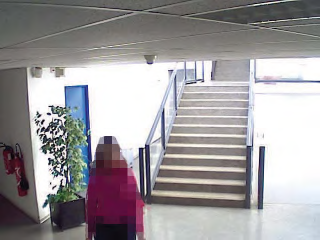
\includegraphics[width=2.0in]{img/sth}%
\label{fig_screen_welcome}}
\hfil
\subfloat[Select equipment screen]{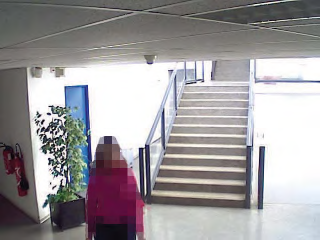
\includegraphics[width=2.0in]{img/sth}%
\label{fig_screen_select_equipment}}
\hfil
\subfloat[Select exercise screen]{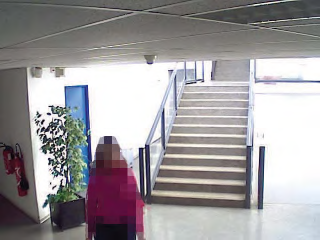
\includegraphics[width=2.0in]{img/sth}%
\label{fig_screen_select_exercise}}
\\
\subfloat[Start exercise screen]{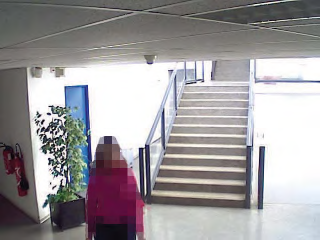
\includegraphics[width=2.0in]{img/sth}%
\label{fig_screen_start_exercise}}
\hfil
\subfloat[Execute exercise screen]{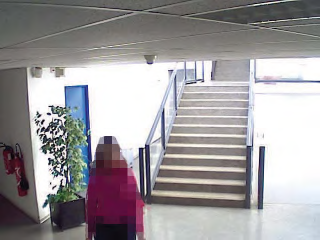
\includegraphics[width=2.0in]{img/sth}%
\label{fig_screen_execute_exercise}}
\hfil
\subfloat[Summany Screen]{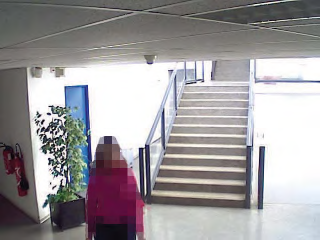
\includegraphics[width=2.0in]{img/sth}%
\label{fig_screen_summary}}
\caption{Screenshots from our application.}
\label{fig_screenshots}
\end{figure*}
%Welcome, SelectEquipment, SelectExercise, StartExercise, ExecuteExercise, Summary

Finally, the user can continue and perform more exercises and log out from the system when he is done with his training. At a later point, for example at home or during the next training session, the user can access all information of all previous trainings in an online interface with a computer or smartphone. In our prototype, a table summarizing all sets and some graphs are included. You can see the web interface in figure \ref{fig_web_screenshot}.

\begin{figure*}[!t]
\centering
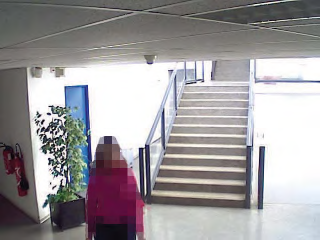
\includegraphics[width=\textwidth]{img/sth}
\caption{Screenshot from the web interface. %TODO explain
}
\label{fig_web_screenshot}
\end{figure*}

\section{Implementation}

First, we are going to describe what components make up our system and how they interact. Then we are describing each component in an own sub-section.

\subsection{Components}
The components that play together to build our application are:
\begin{itemize}
	\item the .NET Gadgeteer, functioning as a bracelet during the workout sessions.
	\item a web server that saves the workout information 
	\item  a web client that and displays all information in a table and graphs.
\end{itemize}

Both the Gadgeteer and the web client access the server that offers a HTTP RESTful interface. The Gadgeteer requests data of available exercises  and uploads the session information. The web client requests this information and displays it in a table and graphically.

\subsection{.NET Gadgeteer}
%TODO rephrase
.NET Gadgeteer as mentioned it is used as a bracelet during the workout session, being so it consists of several components both hardware wise so as software wise. 

\subsubsection{Hardware Components}

This section explains what hardware components of the Gadgeteer we are using and what role they play in our application.

\begin{description}
\item[Accelerometer] plays the main role in our application. After prompting the user to get ready to start a workout, we calibrate the sensor; afterwards we read continuously from the sensor. This sensor data is processed to count repetitions and determine correct performance of the exercise by the software.
\item[WiFi Module] is used immediately when the application starts, connecting to the wireless network created specifically for the components of our application. 
\item[RFID Reader and RFID Tags] help us identifying different users and kinds of equipment.
\item[Display and Tunes Module] are used to give live feedback to the user. We display the numbers of repetitions, and other visual feedback as mentioned in the application flow, and we also use the tunes module to play different notes depending on the correctness of exercise. The display is also used to navigate through our application by touching buttons displayed on it.
\item[Battery] is used so that our application can be used completely wireless.
\end{description}

\subsubsection{Software Architecture}

We organized our software code in packages separating different concerns. Some of them deserve more focus than the others; we will list them all but describe thoroughly the important ones:

\begin{description}
\item[Controller] represent the high level policy of the application. Here we have the \texttt{AppController} class which represent the state manager; it contains the Session which is mutated throughout the application flow. The main thing this AppController does is the switching between different \texttt{ExectuionStates}. It starts with the \texttt{WelcomeState} where it prompts the user to scan their RFID card; and it ends with the \texttt{SummaryState} where it gives a visual feedback about the number of repetitions done. Every \texttt{ExecutionState} has access to hardware events and modules: it has the ability to draw on the display and also to listen and subscribe for different hardware events which can be of interest for that particular state. For instance \texttt{SelectEquipmentState} is interested in the RFID Reader events so that it can process further with identifying the equipment for that particular scanned RFID. 

Every state is an \texttt{ExecutionState} so it contains an \texttt{init()} and \texttt{finish()} method which are called every time the \texttt{AppController} switches between states: where first the \texttt{finish()} of the old state is invoked and afterwards the \texttt{init()} of the new state. Every state paints the display and subscribes for the interested events in the \texttt{init()} and unsubscribes from them in \texttt{finish()}.

\item[GUI] contains two different classes. One of them is used for holding some global constants that are used from different states for painting GUI related things. The other class, \texttt{ParameterizedRectangle}, adds behavior to the existing Rectangle class provided by the .NET Gadgeeter library. The only behavior it adds is the possibility to attach data to a GUI Rectangle; so that every time we paint a rectangle, that always represent buttons in our case, we also associate different relevant data.

\item[Model] represents the data model of the whole application. See the Entity Relationship Diagram. %TODO reference

\item[Network] contains the \texttt{NetworkClient} that has the responsibility of connecting to the WiFi network and also encapsulates all the REST invocations that are needed by the .NET Gadgeeter which are: 
\begin{itemize}
	\item Get User by RFID
	\item Get Equipment by RFID 
	\item Post Session
\end{itemize}

\item[Patterns] package contains the most critical part of our solution. Here we process the data that we get from the accelerometer sensor. The most important classes here are \texttt{IActionPattern} and \texttt{ComplexPattern}. The first one defines an interface that contains an event \texttt{onActionDone} and a method \texttt{processAcel(double x, double y, double z)}. The idea behind this interface is that it represents the logical controller when the user starts performing an exercise. Whenever the user is ready and the sensor is calibrated, based on what exercise they have selected we pass the sensor data to the \texttt{processAcel(...)} method of the current instance. Before doing so; first we subscribe to the \texttt{onActionDone} event of that current instance. This event is fired inside the \texttt{processAcel(...)} after some validations are done based on the exercise and the thresholds related to it.

A \texttt{ComplexPattern} represents a complete exercise made up by different \texttt{IActionPattern}s. The \texttt{ComplexPattern} itself implements the \texttt{IActionPattern} and also contains different \texttt{IActionPattern}s instances. For instance the \texttt{BicepCurl} exercise is a \texttt{ComplexPatern} that contains two different \texttt{IActionPatterns}: \texttt{CurlUpPattern} and \texttt{CurlDownPattern}. We pass the data to the \texttt{BicepCurl} and then the \texttt{BicepCurl} passes internally to the different patterns it contains. We also created another interface that represents an exercise in terms of more meaningful information, abstracting from processing sensor data and the internal way of detecting a pattern. This interface is called \texttt{AbstractExercise} and offers possibilities to start and stop an exercise; to subscribe to the \texttt{onRepetitionDone} event, which is fired every time a complete repetition of that exercise is performed, and other functionalities in the Exercise level of abstraction.
\end{description}

\subsection{Web server}

The server is written in Java and provides a simple RESTful HTTP interface. The libraries used are \texttt{jersey} to provide the web services, \texttt{gson} to serialize and deserialize objects, \texttt{eclipselink} as an ORM and \texttt{h2} as a SQL implementation to create and access databases.

The package \texttt{application} provides a main class, \texttt{services} contains classes to provide the different web services, \texttt{persistence} provides access to the database and a method in \texttt{DataManager} to insert some default data into the database, that we are using, and \texttt{data} contains our data model, where classes have JPA annotations so they can be stored in a database.

%TODO include UML class diagram of the data model.

\subsection{Web client}


\end{document}
